\documentclass[a4paper, 12pt]{article}
\usepackage[utf8]{inputenc}
\usepackage[left=3cm, top=3cm, right=2cm, bottom=2cm]{geometry}%ajusta as margens
\usepackage{setspace}
\setlength{\parindent}{1.25cm}%Altera o parágrafo
\usepackage{graphicx}
\usepackage[portuguese]{babel} 
\usepackage{enumitem}
\setlist[itemize]{label=$\star$}
\begin{document}

\begin{center}
    \large
    \textbf{Faculdade de Tecnologia Baixada Santista Rubens Lara\\}
    \textbf{Curso Superior de Tecnologia em Ciência de Dados}
    \vspace{6.5cm}\\
    Anderson Portes do Nascimento\\Kaylane Chavier Costa\\
    \vspace{6cm}
    \textbf{Álgebra Linear - Algoritmo de Similaridade entre Documentos}
    \\
    \vspace{6cm}
    Santos, SP\\
    2023
\end{center}

\newpage
    \onehalfspacing
    \section{Introdução}
    
    \par O tema escolhido para desenvolvimento do trabalho foi músicas. Através de uma pesquisa bibliográfica, foi encontrado um dataset das 50 principais músicas do Spotify de 2010 a 2019. Baseado neste dataset, o usuário escolhe uma música e o algoritmo recomenda outras através da similaridade entre vetores.



\section{Codificação}

\subsection{Passo 1 - Baixar o Dataset}

\\Foi baixado o arquivo csv do dataset que contém as 50 principais músicas do Spotify de 2010 a 2019. Acessando o link acessando o link: https://gist.github.com/rioto9858/ff72b
72b3bf5754d29dd1ebf898fc893#file-top50musicfrom2010-2019-csv, baixou-se o arquivo na extensão .zip do repositório, no qual foi descompactado na pasta do projeto e, para facilitar o desenvolvimento, renomeado como "musics.csv".

\subsection{Passo 2 - Criar um arquivo Jupyter notebook}

\\Criou-se um arquivo .ipynb (Jupyter notebook) para desenvolver a base do algoritimo.

\subsection{Passo 3 - Importar as bibliotecas que serão utilizadas}

\\Importou-se as bibliotecas que serão utilizadas no desenvolvimento no arquivo .ipynb:

\begin{itemize}
  \begin{description}
    \item[import pandas as pd:] Para realizar a leitura do dataset e modificações;
    \item[from sklearn.feature import CountVectorizer:] Classe usada para "vetorizar" as informações do dataset;
    \item[from sklearn.metrics.pairwise import cosine_similarity:] Função usada para achar a similiaridade entre os vetores;
    \item[import pickle:] Biblioteca usada ao final do algoritimo para guardar variaveis na memória ROM do computador.
  \end{description}
\end{itemize}

\newpage

\subsection{Passo 4 - Importar a base de dados realizar a limpeza das informações}

\\Na segunda célula, fez-se a importação da base de dados e guardou-se na variavel musics. A função read csv espera uma string contendo o caminho do arquivo .csv e retorna uma classe DataFrame da biblioteca pandas.

\\Na terceira célula, a função dropna remove colunas que tenham valores nulos.

\\Na quarta célula, os valores das linhas são renomeados para facilitar posteriormente o desenvolvimento.

\\A quinta célula remove os espaços das strings das linhas de "artist" e "genre" para que, posteriormente, a vetorização ocorra de maneira correta.

\\Por último, utiliza-se a função set value para formatar os valores das colunas. No final, todas terão o prefixo com o nome da sua linha, por exemplo:

\\\\genre artist year == genre:pop artist:artista year:2020

\\pop artista 2020 ==

\\\\Isso é feito para que a função de similiaridade verifique apenas os valores das próprias colunas, como, por exemplo, "bpm" por "bpm" e "artist" por "artist".

\\Além disso, é gerado uma nova linha "tags" contendo a concatenação das linhas do array "keys".

 \begin{figure}[!ht]
        \centering
        \caption{Código do 4º passo}
        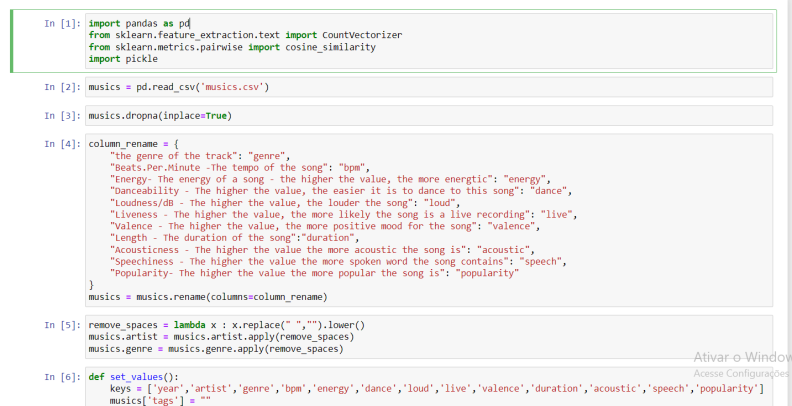
\includegraphics[scale=0.5]{4passo.png} \\
        {\footnotesize Fonte: Elaborada pelo autor.}
        \label{fig:my_label}
    \end{figure}

     \begin{figure}[!ht]
        \centering
        \caption{Código do 4º passo}
        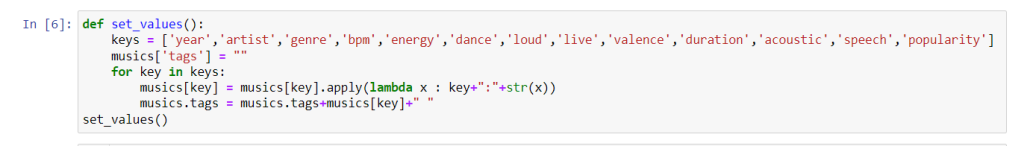
\includegraphics[scale=0.5]{4passo2.png} \\
        {\footnotesize Fonte: Elaborada pelo autor.}
        \label{fig:my_label}
    \end{figure}

\newpage
\subsection{Passo 5 - Vetorização e similaridade}

\\Na 7° célula, foi criada a variável data contendo as colunas "title artist genre" e "tags da variavel musics", automaticamente,
o valor dessa variável se torna uma class "DataFrame" da biblioteca pandas.

\\A variável "count v" da oitava celula se trata de uma instância da classe "CountVectorizer", que será responsável por vetorizar nossos
valores com base nas palavras da linha "tags" das musicas, os vetores foram guardados na variável "vectors".

\\Na célula 10, tem-se a variável "similarity" que representa uma matriz contendo a similiaridade entre cada vetor do dataset.
Nota-se que, quando o valor é 1, se trata de uma comparação com o próprio vetor.
\\\\
1 - [1,...]\\
2 - [...,1,...]\\
3 - [...,...,1]
\\

\\E, assim, sucessivamente. Ou seja, o primeiro elemento do segundo vetor da variavel similarity se trata da comparação da segunda entre a primeira música.
 \begin{figure}[!ht]
        \centering
        \caption{Código do 5º passo}
        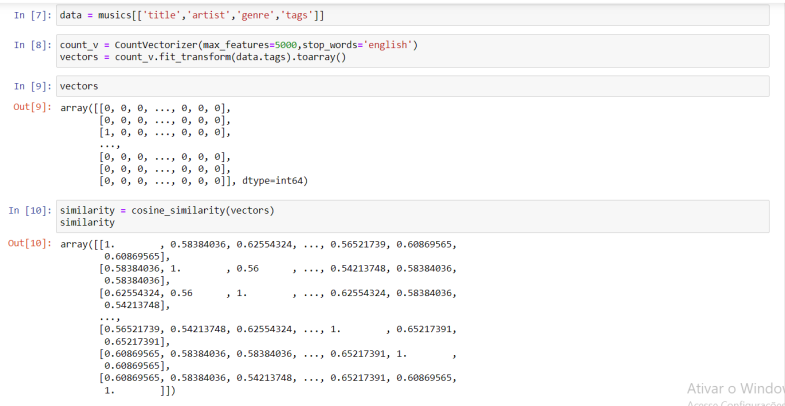
\includegraphics[scale=0.5]{5passo.png} \\
        {\footnotesize Fonte: Elaborada pelo autor.}
        \label{fig:my_label}
    \end{figure}

\subsection{Passo 6 - Função de recomendação}

A função "recommend" espera o nome da música e apresenta o nome de 5 músicas recomendadas.

\\Na primeira linha da função, procura-se pelo índice da música com base no seu nome. O atributo "index" retorna uma tupla com o primeiro valor sendo o índice da coluna, por isso, deve-se usar o [0] para ter somente o índice.

\\Tendo o indice da música, pode-se acessar o vetor de similiaridade usando a variavel "similarity". Para facilitar o entendimento,
guarda-se as músicas com seu índice dentro da variável "musics with index".

\\Por fim, cria-se a variável "musics list" que ordenará as músicas em ordem decrescente, passando o reverse = True e usando o segundo
índice dos elementos da variável "music with index", que será o valor da similiaridade da música.

\\O [1:6] filtra os valores entre menor que 1 e maior que 0.6. Assim, descarta-se a similiaridade da própria música, que seria 1, e remove-se as similiaridades baixas.

\\Dentro do "for", são printados os nomes das músicas recomendadas. Rodando a função usando a música Diamonds, da Rihanna, nota-se
que, dentro das recomendações, tem-se uma música da mesma cantora, a música Work.

 \begin{figure}[!ht]
        \centering
        \caption{Código do 6º passo}
        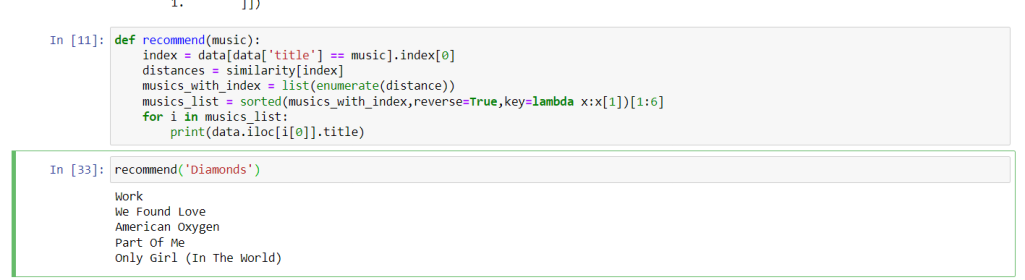
\includegraphics[scale=0.5]{6passo.png} \\
        {\footnotesize Fonte: Elaborada pelo autor.}
        \label{fig:my_label}
    \end{figure}

\subsection{Passo 7 - Armazenar as variáveis}

\\Usando a biblioteca "pickle", armazena-se as variáveis contendo as músicas e similiaridades para usar-se em um novo código. A função dump cria um arquivo da variável passada como primeiro parâmetro e o arquivo passado como segundo parâmetro usando a função "open" nativa do python.

\subsection{Passo 8 - Front-end}

\\Para criar a interface de usuário, é necessário criar um arquivo ".py" no mesmo diretório do projeto para usar as variáveis em
memória geradas pelo "pickle". Após isso, importa-se as seguintes bibliotecas:

\begin{itemize}
  \begin{description}
    \item[import streamlit as st:] Para criar a interface;
    \item[import pickle:] Para ler as variaveis em memória;
    \item[import pandas as pd:] Para importar a base de dados.
  \end{description}
\end{itemize}

\subsection{Passo 9 - Importar base e recriar função de recomendação}

\\Nas linhas 4 a 7 são importadas as variáveis em memória dos arquivos ".pkl" e gerada a classe "DataFrame" das músicas.

\\Na linha 10 a 20 foi recriado a função "recommend", apenas mudando o tipo de retorno para "array", sendo possível apresentar
a música, posteriormente, ao usuário dentro do front-end.

 \begin{figure}[!ht]
        \centering
        \caption{Código do 9º passo}
        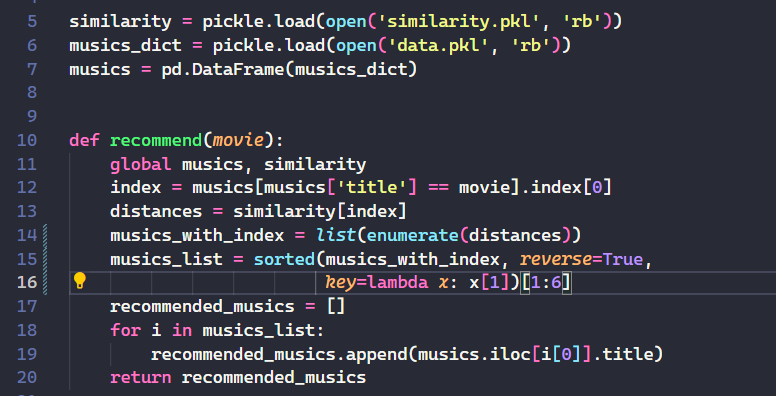
\includegraphics[scale=0.5]{9passo.png} \\
        {\footnotesize Fonte: Elaborada pelo autor.}
        \label{fig:my_label}
    \end{figure}
    
\newpage

\subsection{Passo 10 - Codificação do front-end}
Na linha 23, define-se o título da página como "Music Recommender System".

\\Na linha 24, cria-se um select com o placeholder "Select the music", contendo a lista de músicas do dataset.

\\Na linha 29, é criado um botão que, ao ser clicado, roda a funcão "recommend", passando o valor da música selecionada e, posteriormente,
escrevendo o retorno na tela, para que seja mais seguro ao usuário que tem os valores corretos dos nomes das músicas.

\\Para rodar o front-end, basta digitar no cmd:

\\\\

streamlit run nome-do-arquivo.py
\\\\
Com a biblioteca STREAMLIT instalada. Comando para instalar a biblioteca:
\\\\
-- pip install streamlit
 \begin{figure}[!ht]
        \centering
        \caption{Código do 10º passo}
        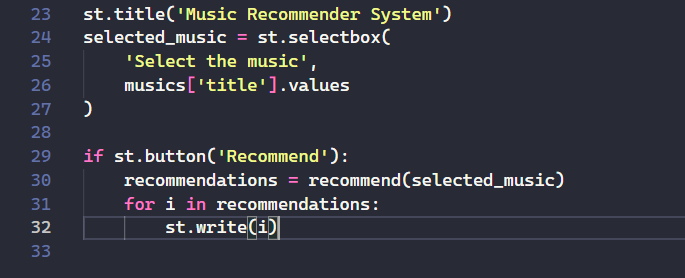
\includegraphics[scale=0.5]{10passo.png} \\
        {\footnotesize Fonte: Elaborada pelo autor.}
        \label{fig:my_label}
    \end{figure}
    
\newpage

\section{Resultado}
Foi criada uma tela para o usuário inserir no input a música escolhida e exibe-se, no output, as músicas recomendadas pelo algoritmo.
\begin{figure}[!ht]
        \centering
        \caption{Resultado}
        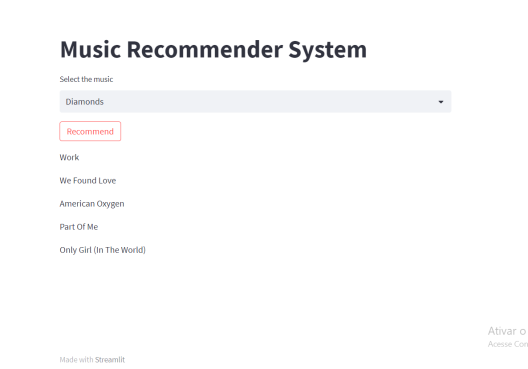
\includegraphics[scale=0.5]{resultado.png} \\
        {\footnotesize Fonte: Elaborada pelo autor.}
        \label{fig:my_label}
    \end{figure}

\begin{figure}[!ht]
        \centering
        \caption{Resultado}
        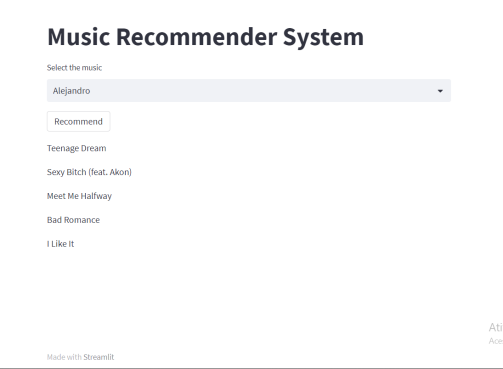
\includegraphics[scale=0.5]{resultado2.png} \\
        {\footnotesize Fonte: Elaborada pelo autor.}
        \label{fig:my_label}
    \end{figure}

\newpage

\section{REPOSITÓRIO DO PROJETO}
Anderson Portes do Nascimento:
    \url{https://github.com/Anderson-Portes/music-recommender}
\\\\Kaylane Chavier Costa:
    \url{https://github.com/kaychavier/music-recommender}
\\\\Dataset:
\url{https://gist.github.com/rioto9858/ff72b72b3bf5754d29dd1ebf898fc893}
\end{document}
%